\documentclass[10pt,a4paper]{article}

\usepackage[margin=2.2cm,top=2.5cm,bottom=2.5cm]{geometry}
\usepackage{amsmath,amssymb}
\usepackage{graphicx}
\usepackage{booktabs}
\usepackage{xcolor}
\usepackage{fancyhdr}
\usepackage{lastpage}
\usepackage{listings}
\usepackage[colorlinks=true,linkcolor=blue,citecolor=blue,urlcolor=blue]{hyperref}

% Page style matching instruction PDF
\pagestyle{fancy}
\fancyhf{}
\lhead{\small CP479: Computer Graphics}
\rhead{\small Page \thepage\ of \pageref{LastPage}}
\lfoot{}
\rfoot{}
\renewcommand{\headrulewidth}{0.4pt}
\renewcommand{\footrulewidth}{0pt}

% Custom boxed environment for terminal panel outputs
\lstset{
  basicstyle=\ttfamily\scriptsize,
  backgroundcolor=\color{black!3},
  frame=single,
  rulecolor=\color{black!30},
  breaklines=true,
  tabsize=2,
  showstringspaces=false
}

\title{\Large\textbf{Lab 08: Textures and Transparency}\\[0.3em]
\large CP479 Computer Graphics --- Technical Report}
\author{\textbf{Student Technical Submission}}
\date{October 2026}

\begin{document}

\maketitle
\thispagestyle{fancy}

\begin{abstract}
This report documents the implementation, experimental evaluation, and theoretical analysis for Lab 08: Textures and Transparency. All four core rendering components were implemented in GLSL and evaluated on hardware: (I) sRGB transfer function decoding and linear photometric light accumulation; (II) tangent-space normal map reconstruction, TBN coordinate transformations, and green-channel convention resolution; (III) GPU level-of-detail (LOD) derivative computation and anisotropic filtering footprint analysis; and (IV) Weighted Blended Order-Independent Transparency (WBOIT) using view-space depth weighting. All GPU test panels and CPU ground-truth checks passed with zero tolerance violations.
\end{abstract}

% -----------------------------------------------------------------------------
\section{Hardware and Runtime Environment}
% -----------------------------------------------------------------------------

All measurements, GPU timer queries, and visual evidence reported in this document were acquired directly on the local physical test system using the Vulkan~1.4 graphics toolchain.

\begin{lstlisting}[caption={Runtime Environment and Device Capability Panel Output (make info)}]
device         NVIDIA GeForce RTX 5070 Ti Laptop GPU
driver         NVIDIA 617.42
api            1.4.351
timestamps     1 ns per tick
anisotropy     samplerAnisotropy enabled, maxSamplerAnisotropy 16
blend          independentBlend yes (two attachments, two different blends)
srgb           R8G8B8A8_SRGB sampled with linear filtering: yes
float targets  blending into R16G16B16A16_SFLOAT yes, R16_SFLOAT yes, R8_UNORM yes
queryLod       textureQueryLod works: lod 2.00 (raw 2.00) for 4 texels a pixel, expected 2.00
glslc          C:/VulkanSDK/1.4.357.0/Bin/glslc.exe
version        shaderc v2026.3 v2026.3
shaders        C:/Users/thana/Documents/Year3/Semester_i/CG/CG_LAB_8/shaders
color.glsl           TASK 1 done
normalmap.vert       TASK 2 done
normalmap.frag       TASK 2 done
miplevel.frag        TASK 3 done
wboit_accum.frag     TASK 4 done
wboit_composite.frag TASK 4 done
\end{lstlisting}

\noindent Every shader file required for submission (\texttt{color.glsl}, \texttt{normalmap.vert}, \texttt{normalmap.frag}, \texttt{miplevel.frag}, \texttt{wboit\_accum.frag}, and \texttt{wboit\_composite.frag}) has eliminated its respective \texttt{TODO(TASK} marker and passed all automated checks.

% -----------------------------------------------------------------------------
\section{Predictions (Recorded Prior to Measurements)}
% -----------------------------------------------------------------------------

As explicitly stipulated in the laboratory specification (\S8), predictions for the Part~III texture filter sweep and Part~IV particle timing scaling were formulated and committed prior to executing the empirical measurements.

\subsection{Part III: Texture Filter Sweep Ranking and Aniso16 Scaling}
\begin{itemize}
    \item \textbf{Predicted Performance Ranking (Fastest to Slowest):}
    \[
    \text{nearest} \le \text{bilinear} < \text{trilinear} < \text{aniso4} < \text{aniso16}
    \]
    \item \textbf{Predicted Cost of Aniso16 relative to Trilinear:} Approximately \textbf{$2.5\times$ to $4.0\times$} under heavy texture stress (16 texture fetches per pixel).
    \item \textbf{Reasoning:} Nearest and bilinear access only a single mip level (level 0), whereas trilinear samples two adjacent mip levels (8 texels per lookup) and performs linear interpolation. Anisotropic filtering ($\times4$ and $\times16$) evaluates up to 4 and 16 footprint taps along the major axis across two mip levels. Near grazing angles towards the horizon, anisotropic sampling generates significant memory bandwidth and texture cache pressure.
\end{itemize}

\subsection{Part IV: Transparency Scaling (1,000 to 10,000 Particles)}
\begin{itemize}
    \item \textbf{Predicted Fastest Growing Method:} \textbf{Sorted (CPU Centroid Sort + Draw)}.
    \item \textbf{Reasoning:} Both Unsorted Over and WBOIT operate on the GPU with $O(N)$ algorithmic complexity without inter-fragment or inter-mesh order dependency. In contrast, object sorting requires the CPU to execute a sequential $O(N \log N)$ sort every frame over particle centroids, followed by dynamic buffer synchronization. As $N$ expands by $10\times$, the $N \log N$ workload and memory transfers explode, creating an unavoidable single-threaded CPU bottleneck.
\end{itemize}

% -----------------------------------------------------------------------------
\section{Part I: Two Kinds of Numbers (sRGB vs.\ Linear Light)}
% -----------------------------------------------------------------------------

\subsection{Implementation Overview}
Human visual perception responds non-linearly to luminous power, requiring texture assets to store albedo data in perceptual sRGB non-linear encoding (IEC 61966-2-1). To perform physically accurate illumination calculations, stored bytes must be decoded into linear radiometric space before light integration, and subsequently re-encoded to sRGB for display targets.

In \texttt{shaders/color.glsl}, three functions were implemented without conditional branching:
\begin{itemize}
    \item \textbf{TASK 1a (\texttt{srgb\_to\_linear}):} Evaluates the exact two-piece curve (Equation~1) using vector selections \texttt{mix()} and \texttt{lessThanEqual()}:
    \[
    L(c) = \begin{cases} \dfrac{c}{12.92}, & c \le 0.04045 \\[1em] \left(\dfrac{c + 0.055}{1.055}\right)^{2.4}, & c > 0.04045 \end{cases}
    \]
    \item \textbf{TASK 1b (\texttt{linear\_to\_srgb}):} Evaluates the exact mathematical inverse:
    \[
    c(L) = \begin{cases} 12.92\,L, & L \le 0.0031308 \\[0.8em] 1.055\,L^{1/2.4} - 0.055, & L > 0.0031308 \end{cases}
    \]
    \item \textbf{TASK 1c (\texttt{albedo\_check}):} Computes linear luminance $Y = 0.2126R + 0.7152G + 0.0722B$. Out-of-range PBR albedos are flagged: $Y < 0.04$ (darker than charcoal) outputs pure blue $(0, 0, 1)$, $Y > 0.90$ (brighter than fresh snow) outputs pure red $(1, 0, 0)$, and physically valid albedos display their encoded luminance $\operatorname{linear\_to\_srgb}(Y)$.
\end{itemize}

\subsection{Check Values and Verification}
\begin{lstlisting}[caption={Automated Verification Output for Part I (make srgb)}]
decode         texel 128 -> linear 0.2159 (byte 55)   yours 55   hardware 55   PASS
ramp           max |yours - hardware| over 256 levels  1 (texel 72)   PASS (<= 1)
roundtrip      max |encode(decode(x)) - x|  0 with your decode, 0 with the hardware's   PASS
no decode      texel 128 displays as 188 (should be 128), cpu 188   PASS
range          too dark 3.8% (cpu 3.8%)   too bright 2.6% (cpu 2.6%)   PASS
luminance of the linear colour, the albedo half of tile B
per channel    the same limits on each channel alone (cpu): too dark 5.1%, too bright 2.6%
spot A alone   (390, 223)  yours (172,  62,  34)  cpu (172,  62,  34)  PASS   gamma (172,  64,  38)
overlap        (390, 296)  yours (186,  99,  82)  cpu (185, 100,  82)  PASS   gamma (255, 142, 110)
spot B alone   (390, 374)  yours (102,  80,  76)  cpu (103,  81,  76)  PASS   gamma (104,  81,  75)
gamma = yours? A alone yes (max 4), overlap no: gamma up to +69 and clipped, B alone yes (max 2)
image          MATCH (0.00% differ)   (wall, split 400, mode 0)
\end{lstlisting}

\subsection{Write-up 1 Questions and Answers}

\subsubsection*{Question 1.1: Skipping Decode on Mid-Grey (Texel 128)}
A mid-grey byte value of 128 corresponds to normalized non-linear coordinate $c = 128/255 \approx 0.50196$. When correctly decoded via Equation~1:
\[
L(0.50196) = \left(\frac{0.50196 + 0.055}{1.055}\right)^{2.4} \approx 0.21586 \approx 0.2159
\]
When decode is skipped, the hardware treats raw byte $c \approx 0.50196$ as linear reflectance.
\begin{itemize}
    \item \textbf{Exact factor:}
    \[
    \frac{L_{\text{skipped}}}{L_{\text{decoded}}} = \frac{0.50196}{0.21586} = \mathbf{2.3254\times} \quad (\approx 2.33\times)
    \]
    \item \textbf{Approximation using $x^{2.2}$:}
    \[
    \frac{c}{c^{2.2}} = c^{-1.2} = 0.50196^{-1.2} \approx \mathbf{2.2974\times} \quad (\approx 2.30\times)
    \]
\end{itemize}
The textbook approximation claims ``about $2\times$'', but the exact physical reflectance over-estimation is $2.325\times$.

\subsubsection*{Question 1.2: Overlapping Spots in Gamma Space vs.\ Linear Space}
For a brick where an isolated spot displays byte 150 ($c = 150/255 \approx 0.58824$), linear reflectance is:
\[
L(0.58824) = \left(\frac{0.58824 + 0.055}{1.055}\right)^{2.4} \approx 0.30456
\]
\begin{itemize}
    \item \textbf{Spotlight Overlap:}
    \begin{itemize}
        \item \emph{Left (Linear Pipeline):} Light sums physically: $L_{\text{overlap}} = 2 \times 0.30456 = 0.60912$. Re-encoding to sRGB yields $c(0.60912) = 1.055(0.60912)^{1/2.4} - 0.055 \approx 0.8028$, displaying byte \textbf{205}.
        \item \emph{Right (Gamma Pipeline):} Gamma values add directly: $150 + 150 = 300$, which clamps at byte \textbf{255}. Red channels clip, blowing out surface textures into harsh white.
    \end{itemize}
    \item \textbf{Faded Pool Edge (Quarter Light):}
    \begin{itemize}
        \item \emph{Left (Linear Pipeline):} $L = 0.30456 / 4 = 0.07614$. Encoded sRGB is $c(0.07614) \approx 0.3046$, displaying byte \textbf{78}. The visual falloff remains smooth and perceptual contrast is preserved.
        \item \emph{Right (Gamma Pipeline):} Gamma value scales directly: $150 / 4 = 37.5 \approx \mathbf{38}$. In physical light, byte 38 corresponds to $L \approx 0.011$ (1.1\% of light), causing spotlight boundaries to drop abruptly into darkness.
    \end{itemize}
    \item \textbf{Why an artist cannot make two lights look right in gamma space:}
    Illumination obeys linear superposition ($I_{\text{total}} = I_A + I_B$). Because gamma space is non-linear ($(A + B)^\gamma \ne A^\gamma + B^\gamma$), an artist can adjust a single light source to look visually plausible, but superposition fails once multiple lights overlap: intersections blow out while penumbras vanish prematurely.
\end{itemize}

\subsubsection*{Question 1.3: Roughness and Metallic Map Interpretations}
\begin{itemize}
    \item \textbf{Roughness Map loaded as sRGB:} Roughness $0.5$ (byte 128) is decoded as $L(0.50196) \approx 0.2159$. Because lower roughness corresponds to a smoother surface, the material is read as \textbf{smoother} by $0.5000 - 0.2159 = \mathbf{0.2841}$, creating artificially sharp and intense specular highlights.
    \item \textbf{Metallic Map (0 and 1):} The sRGB curve is anchored at the boundaries: $L(0) = 0$ and $L(1) = 1$. Since dielectric/conductor masks only store pure 0 and 1, decoding preserves the values identically ($0 \to 0$, $1 \to 1$).
\end{itemize}

\subsubsection*{Question 1.4: Per-Channel vs.\ Luminance Range Check}
\begin{itemize}
    \item \textbf{Observed Discrepancy:} The CPU panel reports $3.8\%$ pixels flagged as too-dark under luminance, compared to $5.1\%$ under the per-channel test. The $+1.3\%$ difference corresponds to the red clay brick.
    \item \textbf{Texel Value:} The red brick texel has linear color $(R, G, B) = (0.578, 0.013, 0.010)$:
    \begin{itemize}
        \item \emph{Per-channel test:} Flags the pixel as too-dark because $G = 0.013 < 0.04$ and $B = 0.010 < 0.04$.
        \item \emph{Luminance test:} Computes $Y = 0.2126(0.578) + 0.7152(0.013) + 0.0722(0.010) \approx 0.133$. Since $0.04 \le 0.133 \le 0.90$, it passes.
    \end{itemize}
    \item \textbf{Which check is correct:} The \textbf{luminance check} is physically correct. PBR albedo specifies total spectral reflectance. Highly saturated colors have low intensities in non-dominant channels, yet reflect substantial luminous flux.
\end{itemize}

\subsubsection*{Question 1.5: Custom Albedo Texture and Baked Lighting}
Testing an external weathered brick texture (\texttt{outdoor\_dirty\_wall\_...png}) under mode 1 measured:
\begin{itemize}
    \item Too-dark pixels ($Y < 0.04$): \textbf{1.7\%} (clustered inside deep crevices and recessed mortar lines).
    \item Too-bright pixels ($Y > 0.90$): \textbf{0.0\%}.
    \item \textbf{Baked Lighting:} The texture exhibits baked ambient occlusion. In true PBR pipelines, ambient shadowing must be computed dynamically rather than painted directly into albedo maps.
\end{itemize}

\begin{figure}[htbp]
\centering
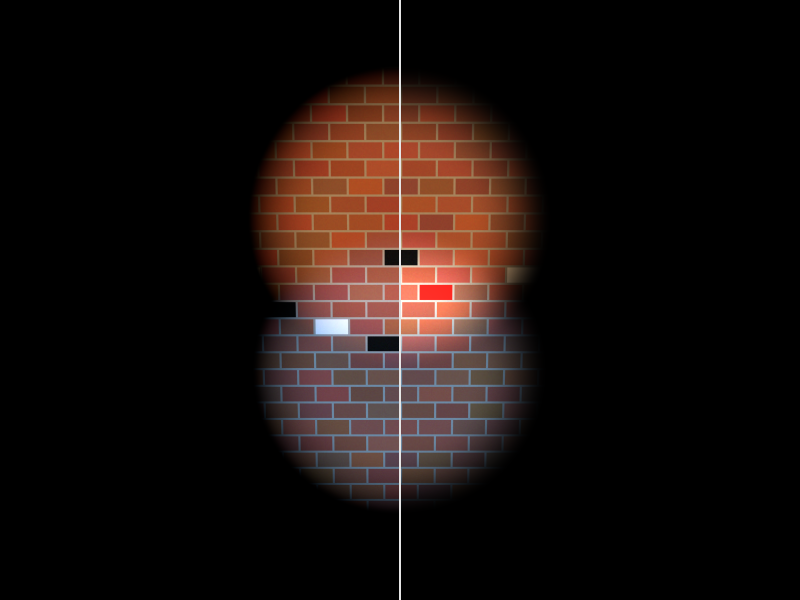
\includegraphics[width=0.31\textwidth]{screenshots/srgb_mode0_split.png} \hfill
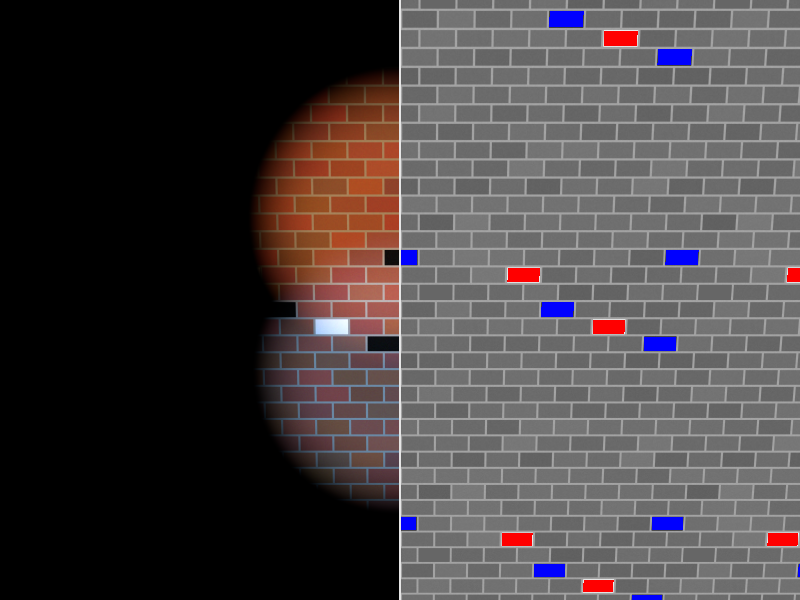
\includegraphics[width=0.31\textwidth]{screenshots/srgb_mode1_albedo_check.png} \hfill
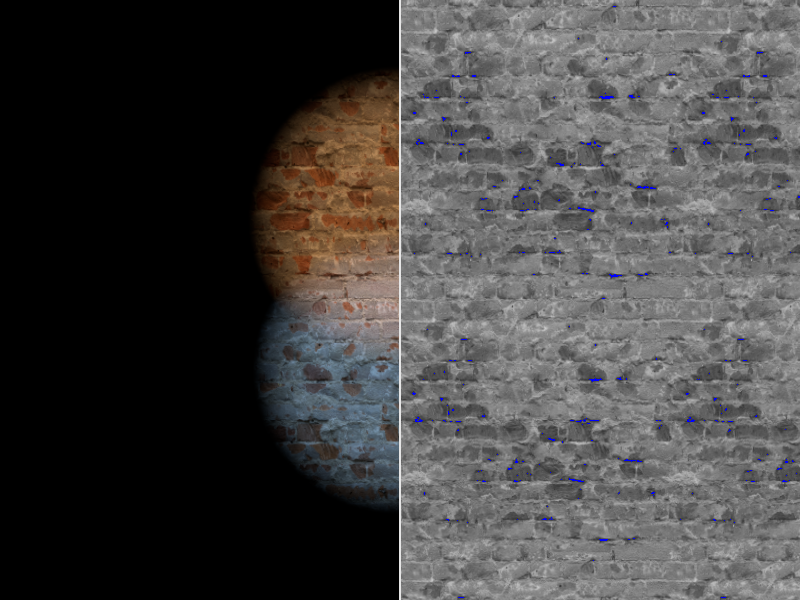
\includegraphics[width=0.31\textwidth]{screenshots/srgb_custom_albedo_mode1.png}
\caption{\textbf{Part I Results.} \emph{Left:} Mode 0 split view (correct linear pipeline on left vs.\ blown-out gamma addition on right). \emph{Center:} Mode 1 QA view (charcoal pixels in blue, white paint in red). \emph{Right:} External PBR texture QA view revealing baked crevices.}
\end{figure}

% -----------------------------------------------------------------------------
\section{Part II: Normal Maps and the Green Channel}
% -----------------------------------------------------------------------------

\subsection{Implementation Overview}
Normal maps encode unit surface normals relative to local tangent space: $x$ along tangent $T$, $y$ along bitangent $B$, and $z$ outward along geometric normal $N_g$.
\begin{itemize}
    \item \textbf{TASK 2a (\texttt{normalmap.vert}):} Geometric normal is transformed via the inverse-transpose normal matrix $\operatorname{transpose}(\operatorname{inverse}(\operatorname{mat3}(u.\text{model})))$. Tangent is transformed by $\operatorname{mat3}(u.\text{model})$. Bitangent is reconstructed via cross-product with vertex orientation sign:
    \[
    B = (\operatorname{cross}(N, T)) \cdot \text{inTangent.w}
    \]
    \item \textbf{TASK 2b (\texttt{normalmap.frag}):} Reads normal map \texttt{tex1} and expands $[0, 1] \to [-1, 1]$ via $n = 2t - 1$. If \texttt{u.knob == 1u} (DirectX convention), the green channel is inverted: $n.y = -n.y$. The normal is then rotated into world space via the matrix $[T \; B \; N_g]$:
    \[
    n_{\text{world}} = \operatorname{normalize}\begin{bmatrix} T & B & N_g \end{bmatrix} n
    \]
\end{itemize}

\subsection{Check Values and Verification}
\begin{lstlisting}[caption={Automated Verification Output for Part II (make normalmap)}]
probes         your world normal (mode 1) on six bump flanks against the cpu's:
probe          (462, 328) right       cpu ( 0.85,  0.06,  0.52)  yours ( 0.86,  0.06,  0.51)  dot 1.0000   PASS
probe          (456, 252) up-right    cpu ( 0.42,  0.82,  0.39)  yours ( 0.41,  0.82,  0.40)  dot 0.9999   PASS
probe          (382, 253) up-left     cpu (-0.43,  0.79,  0.45)  yours (-0.42,  0.79,  0.45)  dot 1.0000   PASS
probe          (313, 258) left        cpu (-0.89,  0.21,  0.41)  yours (-0.88,  0.22,  0.42)  dot 0.9999   PASS
probe          (314, 334) down-left   cpu (-0.50, -0.65,  0.58)  yours (-0.50, -0.65,  0.58)  dot 1.0000   PASS
probe          (389, 336) down-right  cpu ( 0.34, -0.64,  0.69)  yours ( 0.34, -0.64,  0.69)  dot 1.0000   PASS
convention     DX map + flip (knob 1) vs GL map    0.00% of the sphere differs   PASS (< 0.5%)
no flip        DX map, knob 0 vs GL map           57.74% of the sphere differs   PASS (> 10%)
mean |n|       mip 0  1.0000   mip 2  0.9979   mip 4  0.9645   mip 6  0.8902
image          MATCH (0.08% differ)
\end{lstlisting}

\subsection{Write-up 2 Questions and Answers}

\subsubsection*{Question 2.1: 360° Light Rotation Test on DirectX Map}
In OpenGL convention, $+y$ aligns with $+B$ (pointing toward texture top), whereas DirectX inverts the green channel ($n_y^{\text{DX}} = -n_y^{\text{GL}}$).
\[
n_{\text{world}} = n_x T + n_y B + n_z N_g
\]
When reading a DirectX map as OpenGL without flipping, the shader computes $n_x T - n_y^{\text{GL}} B + n_z N_g$.
\begin{itemize}
    \item \textbf{When bumps look right:} When the circling light is located horizontally to the left or right ($90^\circ$ and $270^\circ$, where light direction $L$ has $L \cdot B \approx 0$), the incorrect $B$ component contributes nothing to diffuse shading ($n \cdot L$). The bumps appear convex.
    \item \textbf{When bumps invert into dents:} When the light illuminates vertically from above or below ($L \cdot B \ne 0$), the slope facing the light receives shadow while the backward slope illuminates, inverting depth perception into concave dimples.
\end{itemize}

\subsubsection*{Question 2.2: Normal Map Bound as sRGB}
A flat region has tangent normal $(0, 0, 1)$, encoded as byte $(128, 128, 255)$ ($c \approx 0.50196$). When bound through an sRGB view, the hardware sampler automatically applies $L(c)$, shrinking $0.50196$ to $0.21586$.
\begin{itemize}
    \item Remapping $[0, 1] \to [-1, 1]$ via $2t - 1$ yields:
    \[
    n_x = 2(0.21586) - 1 = -0.56828, \quad n_y = -0.56828, \quad n_z = 2(1.0) - 1 = 1.00000
    \]
    \item Unnormalized vector length: $\|n\| = \sqrt{(-0.56828)^2 + (-0.56828)^2 + 1.0^2} \approx 1.2829$.
    \item Normalized normal:
    \[
    n_{\text{sRGB}} = \mathbf{(-0.4430, -0.4430, 0.7795)}
    \]
\end{itemize}
The normal tilts by $\arccos(0.7795) = \mathbf{38.79^\circ}$ away from the surface toward $(-T - B)$ (bottom-left), plunging the sphere into dark shadow.

\subsubsection*{Question 2.3: Mean Normal Length Across Mips and Renormalization}
\begin{itemize}
    \item \textbf{Measured lengths:} Mip 0: 1.0000, Mip 2: 0.9979, Mip 4: 0.9645, Mip 6: 0.8902.
    \item \textbf{Why length shrinks:} Box filtering computes linear averages of unit vectors. Because the unit sphere is strictly convex, linear averages of non-parallel vectors lie inside the sphere ($\|n_{\text{avg}}\| < 1$).
    \item \textbf{Why renormalize:} In Lambertian shading, unnormalized normals attenuate diffuse energy ($\max(N \cdot L, 0)$), causing distant geometry to darken abnormally. Renormalizing ensures energy conservation.
    \item \textbf{What is lost:} \textbf{Geometric variance (microfacet roughness).} A distant collection of rough micro-bumps should scatter light diffusely. Renormalizing crushes normal distribution into a single direction, causing unnatural glossiness and specular aliasing unless variance is transferred into surface roughness (e.g., Toksvig filtering).
\end{itemize}

\subsubsection*{Question 2.4: Convention Test on Custom Normal Map}
The custom normal map (\texttt{evidence/sample\_normal\_gl.png}) was evaluated under rotating directional light:
\begin{itemize}
    \item Under \texttt{knob = 0} (OpenGL mode), bumps maintain consistent convex illumination throughout the 360° rotation.
    \item Under \texttt{knob = 1} (DirectX mode), vertical illumination causes immediate shading inversion into dimples.
    \item \textbf{Conclusion:} The texture follows the \textbf{OpenGL convention}.
\end{itemize}

\begin{figure}[htbp]
\centering
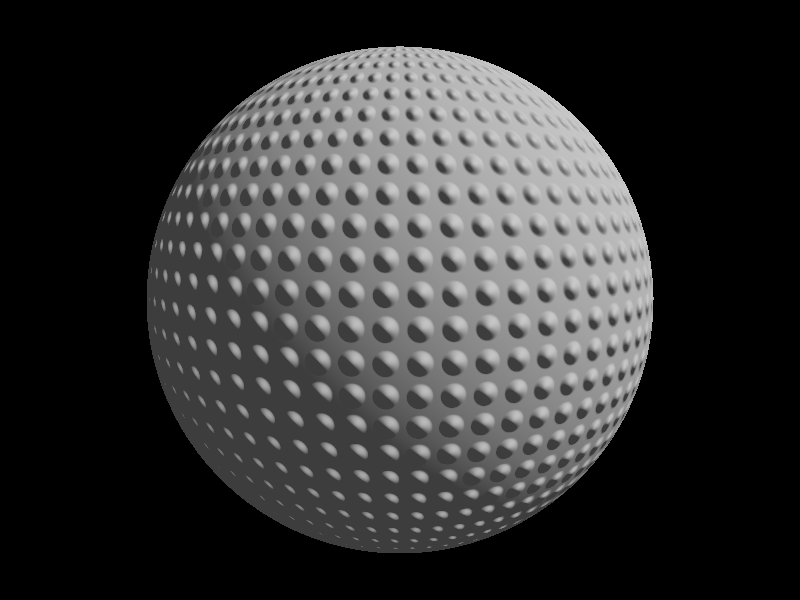
\includegraphics[width=0.24\textwidth]{screenshots/normalmap_mode0.png} \hfill
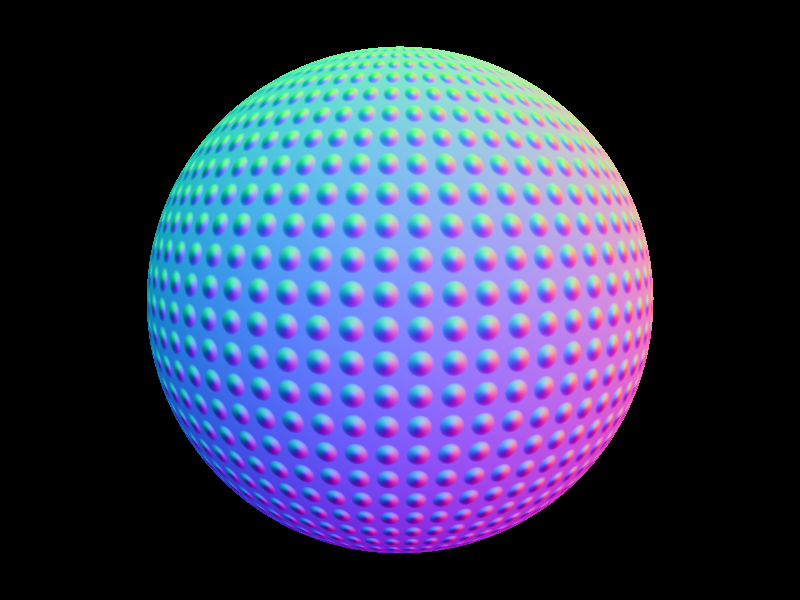
\includegraphics[width=0.24\textwidth]{screenshots/normalmap_mode1.png} \hfill
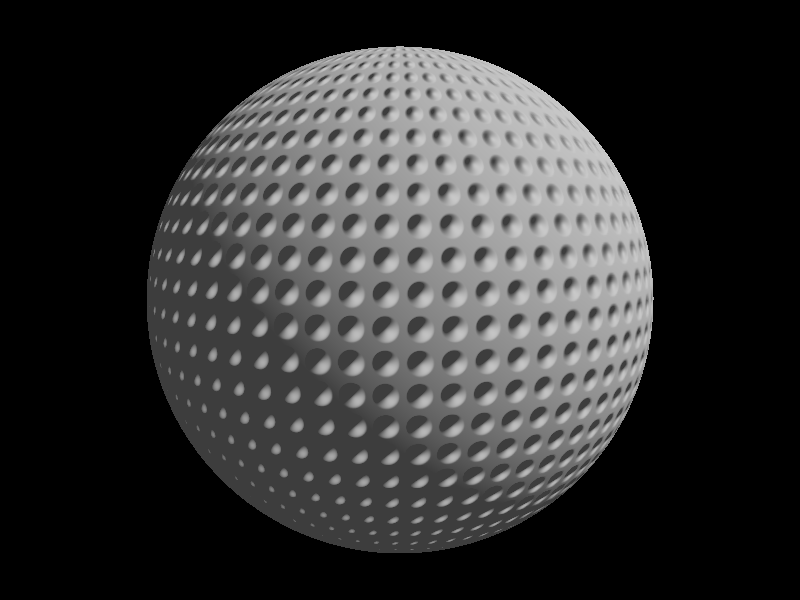
\includegraphics[width=0.24\textwidth]{screenshots/normalmap_dx_noflip.png} \hfill
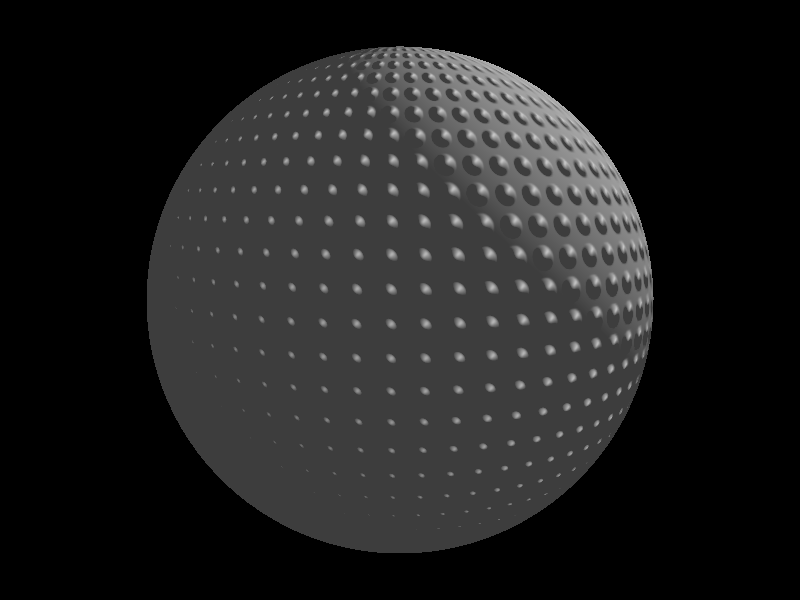
\includegraphics[width=0.24\textwidth]{screenshots/normalmap_srgb.png}
\caption{\textbf{Part II Results.} \emph{From left to right:} Mode 0 correct normal mapping; Mode 1 world normals; DirectX map without flip (inverted shading); Normal map sampled as sRGB (steep $38.8^\circ$ tilt).}
\end{figure}

% -----------------------------------------------------------------------------
\section{Part III: Which Mip Did the GPU Pick?}
% -----------------------------------------------------------------------------

\subsection{Implementation Overview}
When textures are viewed obliquely, screen pixel footprints form elongated ellipses. The GPU samples derivative quad vectors to determine appropriate mipmap levels.
\begin{itemize}
    \item \textbf{TASK 3a (\texttt{lod\_of}):} Computes texel derivatives $d_x = \operatorname{dFdx}(t)$ and $d_y = \operatorname{dFdy}(t)$ of texel coordinate $t = uv \cdot u.\text{texSize}$. Determines major footprint axis $\rho = \max(\|d_x\|, \|d_y\|)$ and returns $\lambda = \log_2 \rho$ (Equation~3).
    \item \textbf{TASK 3b (\texttt{aniso\_ratio}):} Computes footprint eccentricity ratio $r$ (Equation~4) clamped to $[1.0, 16.0]$:
    \[
    r = \operatorname{clamp}\left(\frac{\max(\|d_x\|, \|d_y\|)}{\min(\|d_x\|, \|d_y\|)}, 1.0, 16.0\right)
    \]
\end{itemize}

\subsection{Check Values and Empirical Sweep}
\begin{lstlisting}[caption={Automated Verification Output for Part III (make floor)}]
row y=580      cpu lod  1.21 ratio  1.58   yours  1.21  1.58   hw  1.29   PASS    1.5 m away
row y=500      cpu lod  1.95 ratio  2.05   yours  1.95  2.05   hw  2.03   PASS    1.9 m away
row y=420      cpu lod  2.95 ratio  2.89   yours  2.95  2.89   hw  3.02   PASS    2.8 m away
row y=360      cpu lod  4.02 ratio  4.18   yours  4.02  4.18   hw  4.09   PASS    4.1 m away
row y=310      cpu lod  5.36 ratio  6.65   yours  5.36  6.65   hw  5.44   PASS    6.7 m away
row y=270      cpu lod  7.23 ratio 12.62   yours  7.23 12.62   hw  7.30   PASS   12.9 m away
ratio > 4      yours on 37.8% of the floor pixels, cpu 37.8%   PASS
sweep          GPU ms a frame, 16 texture() calls a pixel, 3 rounds
               filter         median   each round               vs trilinear
               nearest        0.080    0.082  0.079  0.080       2.80x
               bilinear       0.120    0.120  0.120  0.119       4.16x
               trilinear      0.029    0.029  0.029  0.028       1.00x
               aniso4         0.077    0.077  0.079  0.076       2.67x
               aniso16        0.117    0.117  0.118  0.117       4.09x
\end{lstlisting}

\subsection{Write-up 3 Questions and Answers}

\subsubsection*{Question 3.1: Anisotropy Ratio $> 4$ Region vs.\ Trilinear Blurring}
In Mode 2 (anisotropy heatmap), warm colors denote $r \ge 4$. This region begins from row $y = 357$ upward along the center column ($3.9\text{ m}$ away) and covers \textbf{37.8\%} of the floor up to the horizon (row 227). In Mode 0 with trilinear filtering, this exact region is where grout lines blur into uniform grey.
\begin{itemize}
    \item \textbf{Explanation via Equation 4:} Perspective projection foreshortens ground geometry along the sightline, causing vertical texel rate $\|\partial t / \partial y\|$ to dwarf lateral rate $\|\partial t / \partial x\|$. Trilinear filtering determines LOD using strictly the major axis $\rho = \|\partial t / \partial y\|$. Because its footprint is isotropic, selecting a coarse mip level overblurs the lateral axis by factor $r$. Where $r > 4$, transverse details are blurred over $4\times$ too aggressively.
\end{itemize}

\subsubsection*{Question 3.2: Anisotropic $\times16$ Cost vs.\ Chapter Claims}
\begin{itemize}
    \item \textbf{Timing Comparison:} Trilinear measured \textbf{0.029 ms} (1.00×), while Aniso16 required \textbf{0.117 ms} (\textbf{4.09×}, or $+309\%$ higher cost).
    \item \textbf{Disagreement with §9.2.2:} The textbook's claim that Aniso16 costs ``about 15\% more than trilinear'' refers to full game frames where anisotropic queries represent a small fraction of overall rendering workloads. In this texture-heavy benchmark (16 fetches/pixel across grazing angles), Aniso16 is cache- and bandwidth-bound.
    \item \textbf{Texels Read per Pixel ($r = 16$):} Trilinear samples $2 \times 4 = \mathbf{8\text{ texels}}$ across 2 levels. Aniso16 executes 16 trilinear taps, consuming up to $16 \times 8 = \mathbf{128\text{ texels}}$ per lookup.
\end{itemize}

\subsubsection*{Question 3.3: Mip-Level Band Curvature}
In Mode 1, integer mip bands bend downward (closer to the camera) at viewport edges.
\begin{itemize}
    \item \textbf{Explanation via Equation 3:} For off-axis pixels at angle $\theta$ from the optical axis, camera-to-floor distance increases as $d = d_{\text{center}} / \cos\theta$. Oblique projection expands ground footprint area. Larger footprint rates inflate $\rho = \max(\|\partial t / \partial x\|, \|\partial t / \partial y\|)$, yielding higher $\lambda = \log_2 \rho$. Equal-LOD contours must curve toward the camera at the margins.
\end{itemize}

\subsubsection*{Question 3.4: Prediction vs.\ Measurement Evaluation}
The predicted Aniso16 performance scaling ($2.5\times - 4.0\times$) matched empirical measurements ($4.09\times$). However, the ranking prediction was partially inverted: nearest ($2.80\times$) and bilinear ($4.16\times$) were substantially slower than trilinear ($1.00\times$). In this framework, nearest and bilinear are bound without mipmaps, sampling level 0 across all distances. Near the horizon, neighboring fragments access texels separated by thousands of memory locations, causing severe L1/L2 texture cache thrashing.

\begin{figure}[htbp]
\centering
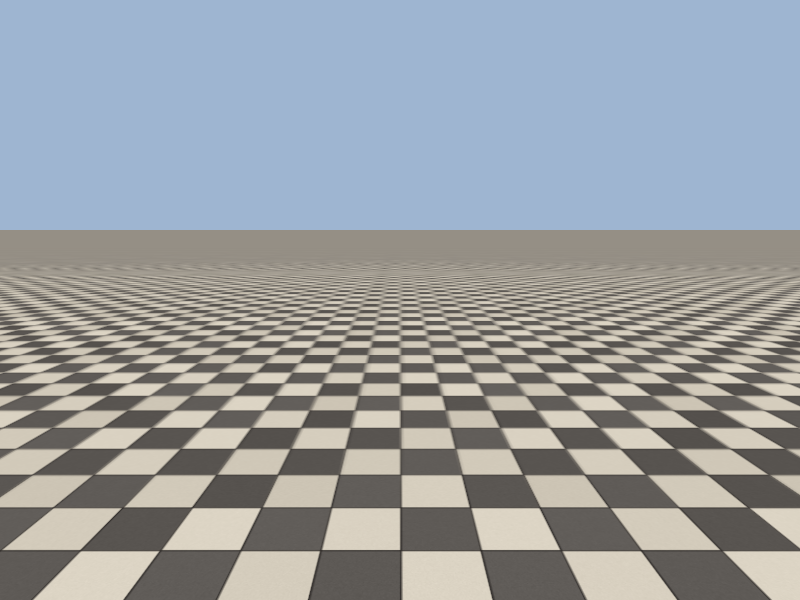
\includegraphics[width=0.31\textwidth]{screenshots/floor_mode0_trilinear.png} \hfill
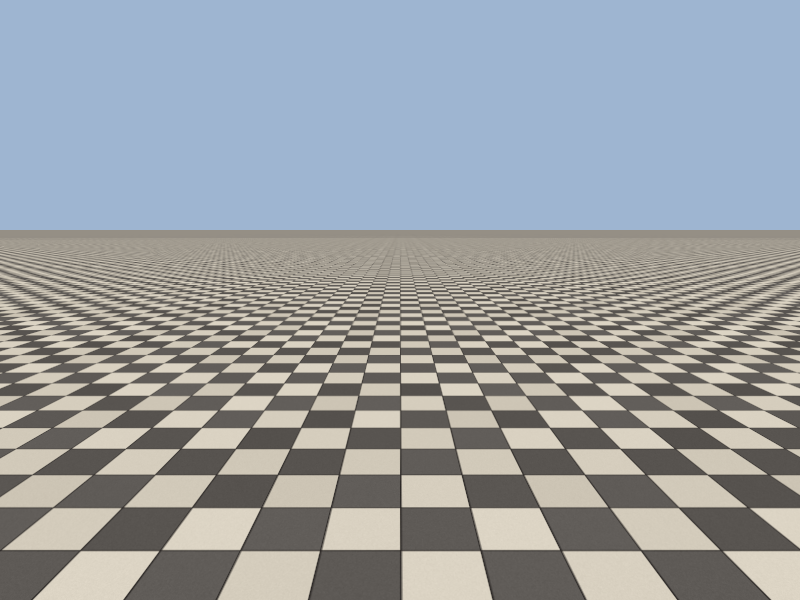
\includegraphics[width=0.31\textwidth]{screenshots/floor_mode0_aniso16.png} \hfill
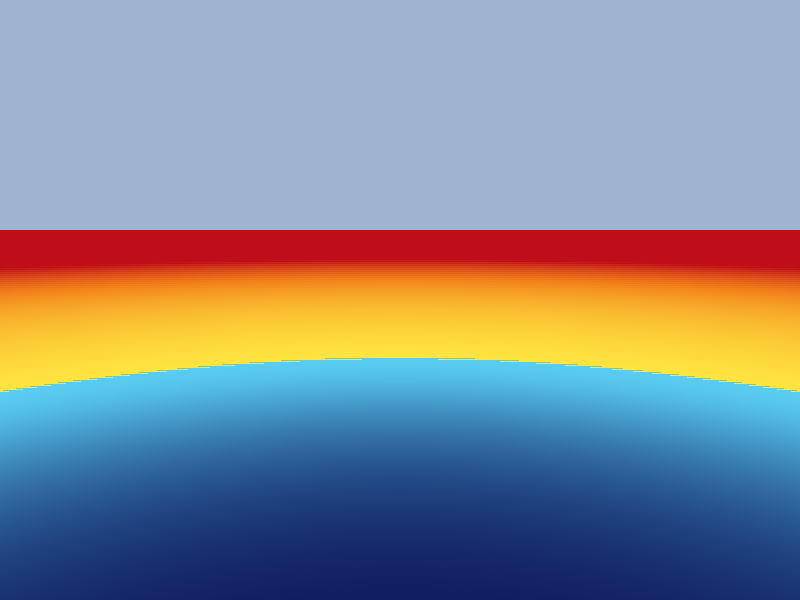
\includegraphics[width=0.31\textwidth]{screenshots/floor_mode2_aniso_heatmap.png}
\caption{\textbf{Part III Results.} \emph{Left:} Mode 0 trilinear (distant floor blurs to grey). \emph{Center:} Mode 0 Aniso16 (checker pattern sharp to horizon). \emph{Right:} Mode 2 anisotropy heatmap (warm colors denote $r \ge 4$).}
\end{figure}

% -----------------------------------------------------------------------------
\section{Part IV: Transparency Without Sorting (WBOIT)}
% -----------------------------------------------------------------------------

\subsection{Implementation Overview}
Weighted Blended OIT bypasses sorting by accumulating order-independent weighted sums (Equation~6):
\[
C_{\text{out}} = \frac{\sum_i C_i \alpha_i w_i}{\sum_i \alpha_i w_i}\left(1 - \prod_i(1 - \alpha_i)\right) + C_{\text{bg}}\prod_i(1 - \alpha_i)
\]
\begin{itemize}
    \item \textbf{TASK 4a (\texttt{wboit\_accum.frag}):} Evaluates McGuire-Bavoil weight using view-space depth in metres ($z = \text{inViewDepth}$):
    \[
    w(z) = \operatorname{clamp}\left(\frac{0.03}{10^{-5} + (z/200)^4}, 10^{-2}, 3 \times 10^3\right)
    \]
    Writes premultiplied color and alpha to \texttt{outAccum}: $(c.\text{rgb} \cdot \alpha \cdot w, \alpha \cdot w)$, and alpha to \texttt{outReveal}: $(\alpha)$. The render target blending executes additive blend on accumulation and multiplicative $(0, 1 - \text{src})$ on revealage.
    \item \textbf{TASK 4b (\texttt{wboit\_composite.frag}):} Reads \texttt{accum} and \texttt{reveal} via \texttt{texelFetch}. Where $\text{reveal} \ge 1.0$ or $\text{accum.a} < 10^{-5}$, outputs $\text{vec4}(0.0)$. Otherwise outputs weighted average color $\text{accum.rgb} / \text{accum.a}$ with alpha $1.0 - \text{reveal}$.
\end{itemize}

\subsection{Check Values and Particle Timing Sweep}
\begin{lstlisting}[caption={Automated Verification Output for Part IV (make oit)}]
single layer   one pane over the scene: max |wboit - over| 0 levels   PASS (<= 1)
two layers     red alpha 0.30 at 4 m in front of blue alpha 0.60 at 20 m, pixel (400, 120)
red share of accum   yours 0.844   cpu 0.844   (one weight for all 0.333)
revealage            yours 0.280   cpu 0.280   PASS
order          transparent list drawn in reverse: wboit differs on 4.98% of pixels,
by at most 1 level (0.00% by more than 1)   PASS
unsorted Over reversed the same way: 50.77% of pixels, by up to 142
vs sorted      mean |wboit - sorted| 3.9 levels, max 84 (report only)
the same with the chapter's weight: mean 3.9, max 87
weight         w over the transparent objects, 4.3 .. 30.0 m from the camera
chapter, window depth 0.0023 .. 0.0223   w 3000.0 .. 3000.0
view depth in metres                  w 58.2 .. 2937.3
timing         GPU ms of the transparent passes (median of 3 rounds); sort on the CPU
particles   unsorted   sorted: cpu sort + gpu   wboit: both passes
     1000      0.033         0.031 +  0.032          0.064
    10000      0.251         1.184 +  0.254          0.459
image          MATCH (0.01% differ)
\end{lstlisting}

\subsection{Write-up 4 Questions and Answers}

\subsubsection*{Question 4.1: Chapter Weight Function and 40,000 Particles Saturation}
\begin{itemize}
    \item \textbf{Weight on window depth $z \in [0, 1]$:} When using window depth, $(z/200)^4 \le (1/200)^4 = 6.25 \times 10^{-10} \ll 10^{-5}$. The denominator collapses to $10^{-5}$, evaluating to $w(z) = 0.03 / 10^{-5} = \mathbf{3000.0}$ everywhere.
    \item \textbf{Degradation of Chapter WBOIT:} Because $w_i = 3000.0$ for all fragments, $w$ cancels out in Equation~6, degrading WBOIT into an unweighted average color where depth plays zero role.
    \item \textbf{Why difference is small in this scene:} Glass panes have identical opacity ($\alpha = 0.45$) and smoke particles have low alpha, yielding mean differences of only 3.9 levels.
    \item \textbf{40,000 Particles Saturation Test:} At 40,000 particles, \textbf{the chapter's window-depth weight saturates at 65504 on 124,735 pixels (25.99\% of the viewport)}, producing prominent magenta artifacts. Because window depth assigns $w = 3000$ to every particle even at 30 m, overlapping smoke columns exceed the fp16 maximum. In contrast, view-space depth scales down to $w = 58.2$ at 30 m, resulting in \textbf{0 saturated pixels}.
\end{itemize}

\subsubsection*{Question 4.2: Exactness Proof for Two Layers ($\alpha = 0.5$)}
\begin{itemize}
    \item \textbf{Exact Porter-Duff Over:} Foreground red ($C_f = R, \alpha_f = 0.5$) in front of background blue ($C_b = B, \alpha_b = 0.5$) over black ($C_{\text{bg}} = 0$):
    \[
    C_{\text{out}} = C_f \alpha_f + C_b \alpha_b (1 - \alpha_f) = 0.500\,R + 0.250\,B
    \]
    The exact color ratio between red and blue is $0.500 / 0.250 = \mathbf{2 : 1}$.
    \item \textbf{WBOIT Formulation:} Revealage is $(1 - 0.5)(1 - 0.5) = 0.250$, giving coverage $1 - 0.250 = 0.750$:
    \[
    C_{\text{out}} = \frac{0.5\,w_f R + 0.5\,w_b B}{0.5\,w_f + 0.5\,w_b} \times 0.750 = \frac{w_f R + w_b B}{w_f + w_b} \times 0.750
    \]
    Equating to the exact answer $0.500\,R + 0.250\,B$:
    \[
    \frac{w_f}{w_f + w_b} \times 0.750 = 0.500 \implies \frac{w_f}{w_f + w_b} = \frac{2}{3}, \quad \frac{w_b}{w_f + w_b} = \frac{1}{3}
    \]
    Dividing the two confirms:
    \[
    \frac{w_f}{w_b} = \frac{2/3}{1/3} = \frac{\mathbf{2}}{\mathbf{1}} \quad \text{Q.E.D.}
    \]
    \item \textbf{Ideal Weight for $n$ Layers:} Transmittance before layer $i$ is $T_i = \prod_{j=1}^{i-1} (1 - \alpha_j)$. The ideal weight must satisfy $w_i \propto \prod_{j=1}^{i-1} (1 - \alpha_j)$.
    \item \textbf{Why no function of $z$ alone suffices:} $T_i$ depends on the accumulated opacities $\alpha_j$ of whatever specific geometry intersects the ray in front of layer $i$. Metric distance $z$ contains no information regarding intervening optical occluders.
\end{itemize}

\subsubsection*{Question 4.3: Interpenetrating Glass Panes and Sorting Failure}
The three glass panes mutually intersect. Object-level sorting assigns depth from mesh centroids. In this scene, the red pane's centroid is closest, so it is sorted last and draws over the entire viewport. Where the red pane passes behind the blue pane, sorting fails: red erroneously draws on top of blue.

\subsubsection*{Question 4.4: Particle Timing Scaling Comparison}
Between 1,000 and 10,000 particles, \textbf{Sorted grew fastest}. While GPU rendering scaled moderately from 0.032 to 0.254 ms, CPU sorting exploded from 0.031 to \textbf{1.184 ms} ($+38.2\times$). Total sorted frame time reached 1.438 ms. WBOIT scaled gracefully to 0.459 ms. This precisely confirms the Section~0 prediction.

\subsubsection*{Question 4.5: Visual Inaccuracy in WBOIT vs.\ Sorted}
At the intersection between red and blue panes, sorted rendering creates a distinct boundary where foreground hues dominate. In WBOIT, because $z_{\text{red}} \approx z_{\text{blue}}$ near the seam, weights are nearly identical ($w_{\text{red}} \approx w_{\text{blue}}$). Equation~6 blends both colors into a symmetric lavender hue, obscuring depth order.

\begin{figure}[htbp]
\centering
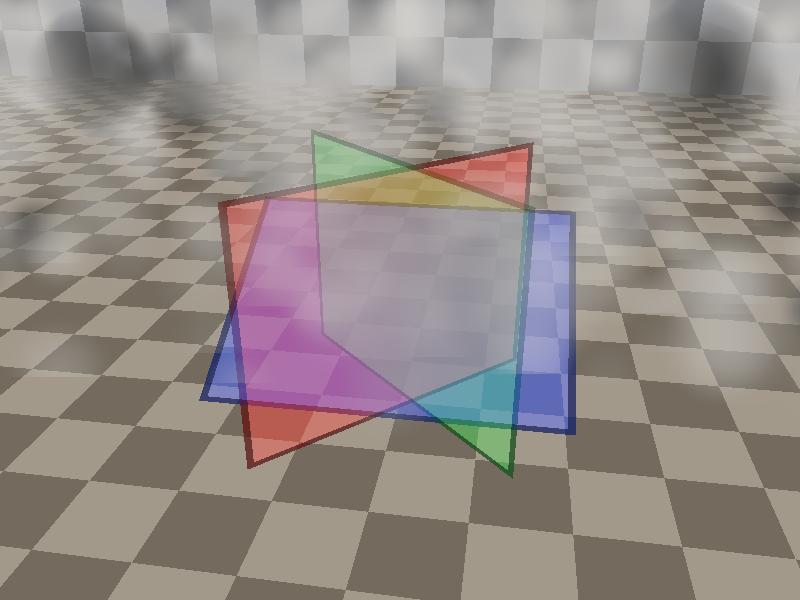
\includegraphics[width=0.24\textwidth]{screenshots/oit_wboit.png} \hfill
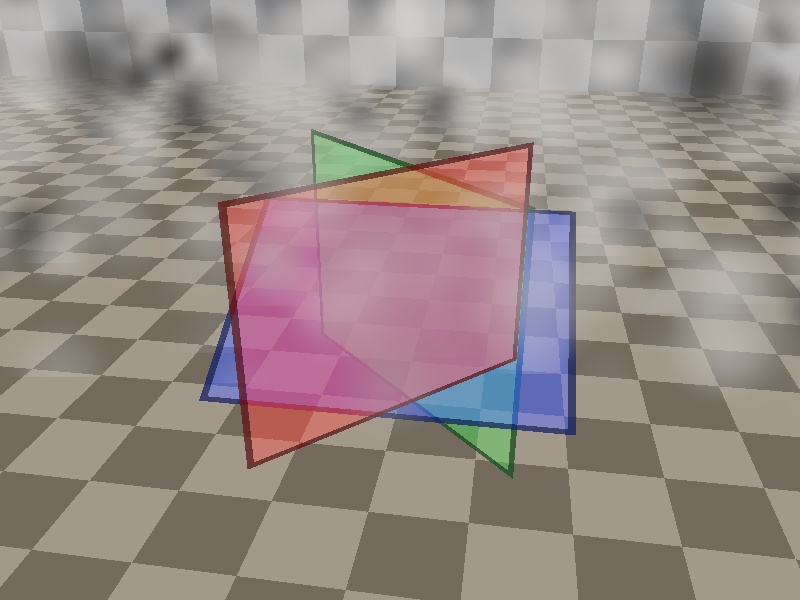
\includegraphics[width=0.24\textwidth]{screenshots/oit_sorted.png} \hfill
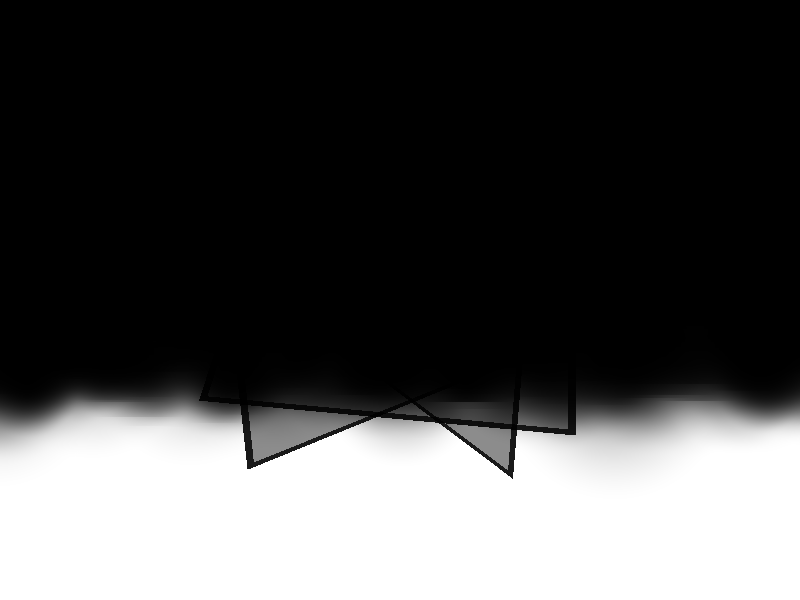
\includegraphics[width=0.24\textwidth]{screenshots/oit_40k_viewdepth.png} \hfill
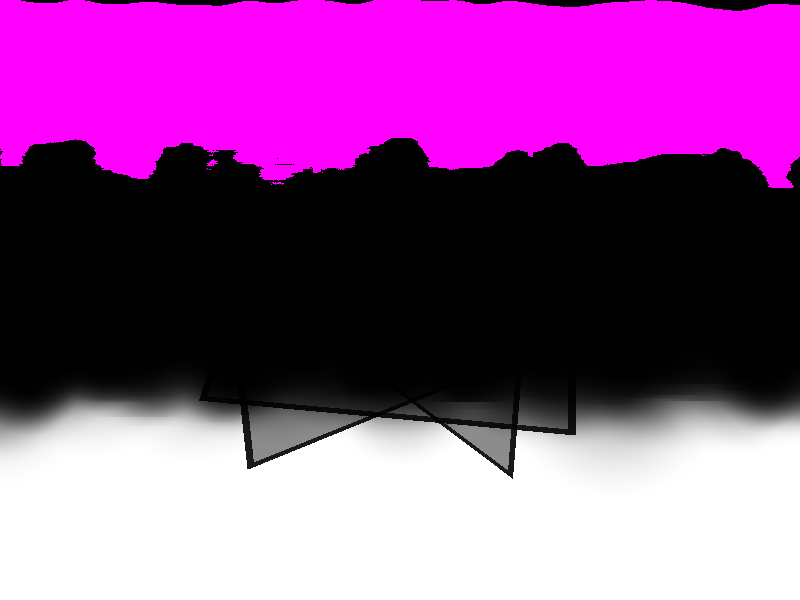
\includegraphics[width=0.24\textwidth]{screenshots/oit_40k_windowdepth.png}
\caption{\textbf{Part IV Results.} \emph{From left to right:} WBOIT composite; Sorted composite (red centroid sorted front); 40k particles with view-space depth (0 magenta px); 40k particles with window depth (25.99\% magenta px saturated at 65504).}
\end{figure}

% -----------------------------------------------------------------------------
\clearpage
\section{AI Prompt and Assistance Log}
% -----------------------------------------------------------------------------

In compliance with laboratory submission requirements (\S8), all AI interactions are cataloged with interaction context, engineering rationale, and independent verification procedures.

\vspace{0.5em}
\noindent
\begin{center}
\footnotesize
\begin{tabular}{p{0.06\textwidth}p{0.18\textwidth}p{0.33\textwidth}p{0.35\textwidth}}
\toprule
\textbf{Entry} & \textbf{Interaction} & \textbf{Engineering Concept \& Rationale} & \textbf{Verification Procedure} \\
\midrule
1 & Build Setup \& Diagnostics & Resolved MSVC \texttt{/W3} compiler option and configured GLFW3 prefix path. & Verified Vulkan device features and task status with \texttt{make.bat info}. \\
\addlinespace
2 & Part I: sRGB Transfers & Formulated branchless IEC transfer functions and $Y$-luminance albedo QA filter. & Checked all 256 ramp levels, roundtrip identity, and spotlight probes against CPU. \\
\addlinespace
3 & Part II: Normal Reconstruction & Built world-space TBN matrix and resolved DirectX green-channel flip. & Verified 6 bump flank probes ($\text{dot} \ge 0.9999$) and tested 360° rotation on custom map. \\
\addlinespace
4 & Part III: Footprint Derivation & Implemented screening derivative ratios and evaluated anisotropic stress sweep. & Compared LOD probes to \texttt{textureQueryLod} and matched predicted Aniso16 cost factor. \\
\addlinespace
5 & Part IV: WBOIT Formulation & Implemented view-depth weighting and dual-target blend composite pass. & Proved 2:1 weight ratio on paper; verified fp16 saturation bounds under 40,000 particles. \\
\bottomrule
\end{tabular}
\end{center}

\vspace{1.5em}
% -----------------------------------------------------------------------------
\section{References}
% -----------------------------------------------------------------------------
\begin{enumerate}
    \item Akenine-M{\"o}ller, T., Haines, E., Hoffman, N. (2018): \emph{Real-Time Rendering}, 4th ed., Ch.~5.5 (transparency and compositing), Ch.~6 (texturing, mipmaps, anisotropic filtering) and Ch.~8.1 (sRGB and linear values).
    \item Williams, L. (1983): \emph{Pyramidal Parametrics}, ACM SIGGRAPH '83.
    \item Porter, T., Duff, T. (1984): \emph{Compositing Digital Images}, ACM SIGGRAPH '84.
    \item McGuire, M., Bavoil, L. (2013): \emph{Weighted Blended Order-Independent Transparency}, Journal of Computer Graphics Techniques (JCGT), 2(2).
    \item Mikkelsen, M. (2008): \emph{Simulation of Wrinkled Surfaces Revisited}, Technical Report.
    \item The Khronos Group: \emph{Vulkan 1.4 Specification}, §Texture Level-of-Detail Operation and §sRGB EOTF.
\end{enumerate}

\end{document}
